Les spécifications du projet ont été définies au début du projet, et réparties en plusieurs versions. L'objectif de ce semestre était d'atteindre la version 1.0 et de développer des fonctionnalités supplémentaires des versions suivantes selon l'avancement du projet.

\section{Besoins détaillés}

\subsection{Spécifications fonctionnelles}

Cette partie présente la liste de toutes les fonctionnalités qu'il aurait été possible d'implémenter dans cette application.

\subsubsection{Version 1.0}

\paragraph{Création de compte, connexion et déconnexion\newline} 

\par Dans la version 1.0, chaque utilisateur a la possibilité de créer un nouveau compte dans l’application grâce à une interface de création de compte. L’utilisateur peut par la suite se connecter sur l’application grâce à son compte via une interface de connexion. Après s'être connecté, il peut aussi se déconnecter. 


\paragraph{Discussion en ligne\newline} 

\par Une fois connecté l'utilisateur peut voir la liste des autres utilisateurs, cette liste contient une mention de si chacun de ces utilisateurs est connecté ou non. Il a ainsi la possibilité d’engager une conversation écrite avec un ou plusieurs utilisateurs connectés. 

\par L’utilisateur peut également voir la liste des conversations effectuées ou en cours, et en reprendre s'il le souhaite. Le fait de reprendre une conversation permet de voir l’historique de celle-ci et d’ajouter de nouveaux messages. 

\subsubsection{Version 2.0}

\paragraph{Discussion audio\newline}

\par La version 2.0 introduit la discussion audio. Cela permet aux utilisateurs d’effectuer des appels audio entre eux. Toutefois cette fonctionnalité n'est possible que pour les conversations par paire.

\paragraph{Contrôle parentale et filtrage\newline}

\par Lors de la création d’un compte ou de la modification de profil, l’utilisateur peut activer ou désactiver le contrôle parental pour pouvoir filtrer les messages ou empêcher les conversations dans certaines fenêtres de temps dans la journée.

\par Ces filtres sont configurables via une interface de configuration de filtrage.

\subsubsection{Version 3.0}

\paragraph{Création d’une IA en tant qu’utilisateur de la messagerie\newline}

\par Une Intelligence Artificielle (IA) apparaît à la version 3.0 de l’application. Cette dernière permet aux utilisateurs "humains" d’avoir une conversation minimaliste.

\paragraph{Image de profil pour chaque utilisateur\newline}

\par Dans le but de différencier les utilisateurs une image de profil peut être ajoutée et est visible de tous les autres utilisateurs.

\paragraph{Avatar 3D lors de la conversation audio\newline}

\par Les conversations audio de base ne donnent pas de feedback aux utilisateurs. Pour palier à ce problème et rendre plus interactive cette discussion l’utilisation d’un avatar 3D sera possible par les utilisateurs.

\paragraph{Affichage d’emoji\newline}

\par Les conversations textuelles ne transmettent pas les différentes émotions simplement (Rire, tristesse, ...). Afin de simplifier cela des “emojis” peuvent être mis en place. 

\newpage
\subsubsection{Cas d’utilisation}

Diagramme de cas d'utilisations : \newline


	\begin{figure}[!h]
		\centering 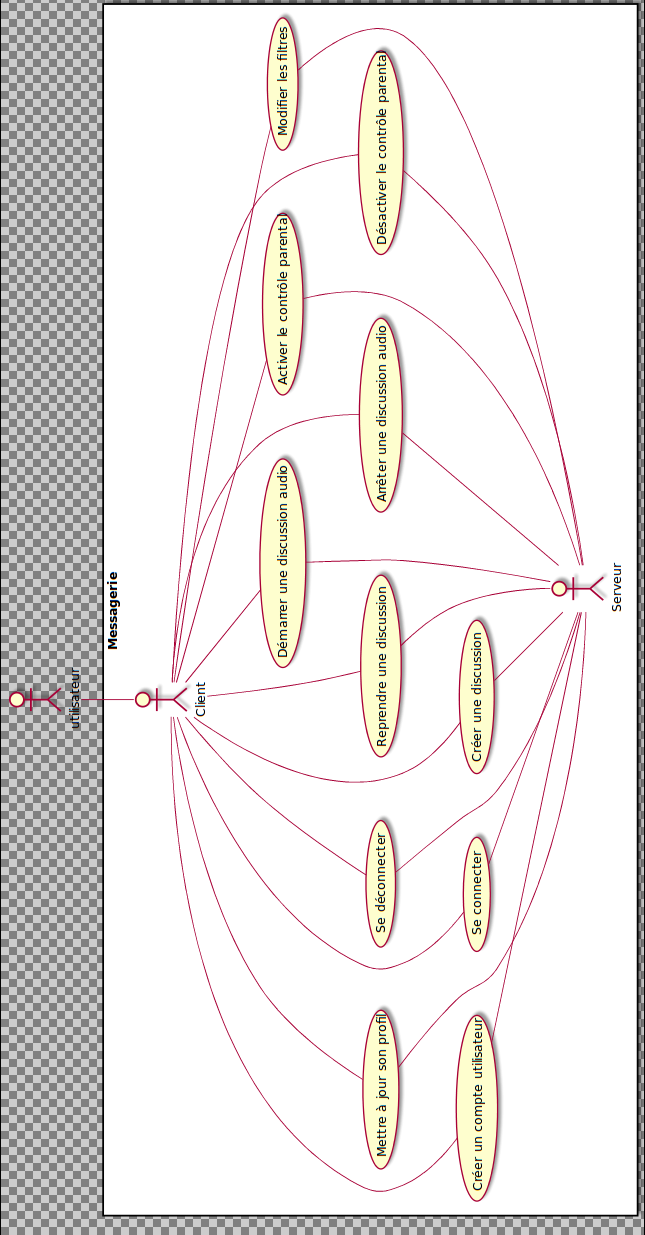
\includegraphics[scale=0.46]{img/usecase.png}
		\caption{Cas d'utilisation}
	\end{figure}
	
	
\subsection{Spécifications d’interface}

\subsubsection{Interface de l’application}

\par L’application doit être responsive design afin d’être consultable autant sur ordinateur, smartphone ou tablette, quelque soit les résolutions d’écrans. 

\par L’interface utilisateur doit être intuitive et facile d’utilisation. 

\subsubsection{Arborescence de l’application web}

\begin{itemize}
	\item Page d'accueil permettant à l’utilisateur de s'inscrire ou de se connecter à la messagerie.	
	\item Une fois connecté, la page principale de la messagerie contenant les éléments majeurs de l'application web tels que la liste des utilisateurs connectés, l’historique des dernières conversations en ligne et son espace membre avec son image de profil ou avatar.
	\item Page de discussion 
	\item Page de configuration du profil
	\item Page de configuration des filtres
\end{itemize}

\subsubsection{Maquettes}

Cette partie présentes les maquettes qui ont été réaliser avant la réalisation. 

\begin{figure}[H]
   \begin{minipage}[c]{.46\linewidth}
      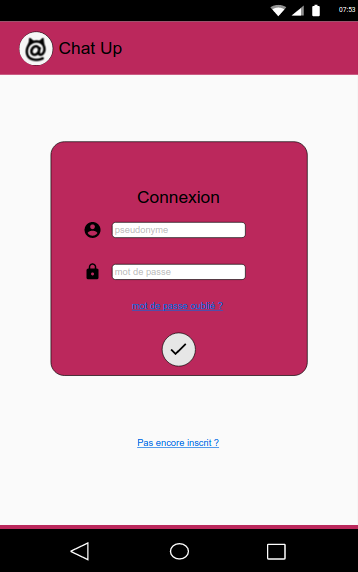
\includegraphics[scale=0.5]{img/SeConnecter.png}
      \caption{Page de connexion}
   \end{minipage} \hfill
   \begin{minipage}[c]{.46\linewidth}
      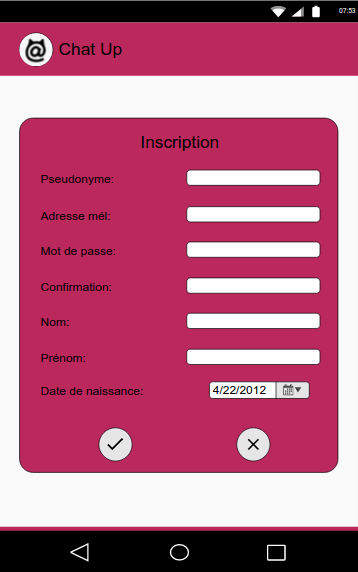
\includegraphics[scale=0.5]{img/CreerUnCompte.png}
      \caption{Page d'inscription}
   \end{minipage}
\end{figure}


\begin{figure}[H]
   \begin{minipage}[c]{.46\linewidth}
		\centering 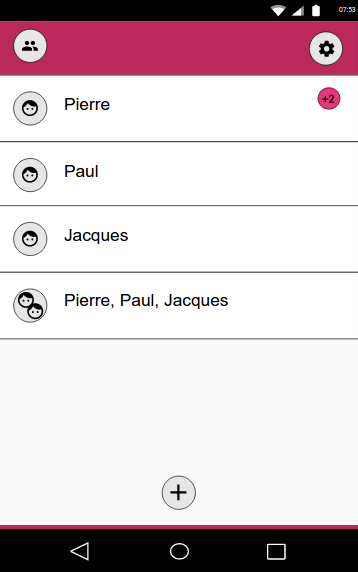
\includegraphics[scale=0.5]{img/Messagerie.png}
		\caption{Page de messagerie}
   \end{minipage} \hfill
   \begin{minipage}[c]{.46\linewidth}
		\centering 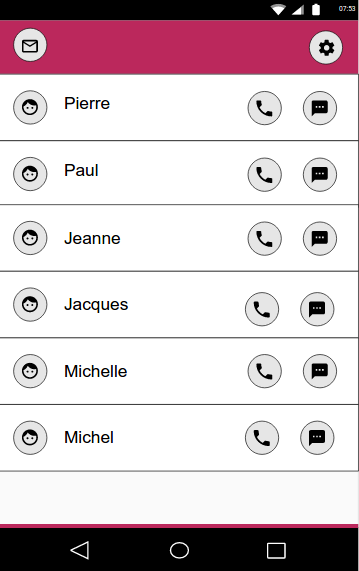
\includegraphics[scale=0.5]{img/Contacts.png}
		\caption{Page des contacts}
   \end{minipage}
\end{figure}

\begin{figure}[H]
   \begin{minipage}[c]{.46\linewidth}
		\centering 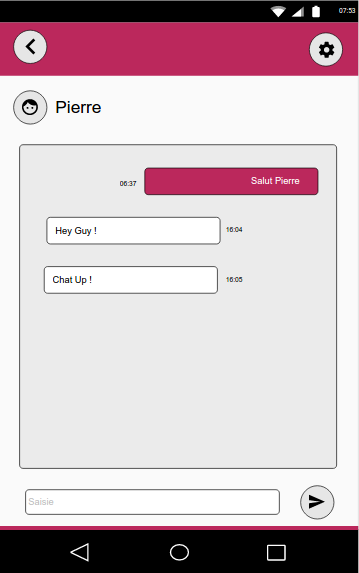
\includegraphics[scale=0.5]{img/Conversation.png}
		\caption{Conversation textuelle}
   \end{minipage} \hfill
   \begin{minipage}[c]{.46\linewidth}
		\centering 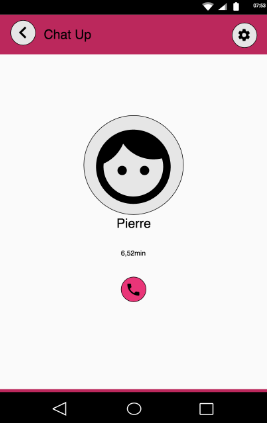
\includegraphics[scale=0.68]{img/audio.png}
		\caption{Conversation audio}
   \end{minipage}
\end{figure}


	\begin{figure}[H]
		\centering 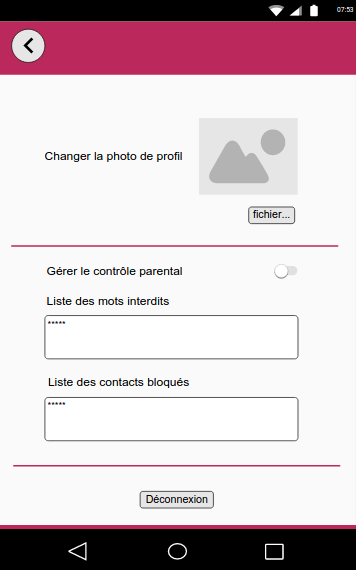
\includegraphics[scale=0.5]{img/Parametres.png}
		\caption{Page de paramètres}
	\end{figure}
	
	
\subsection{Spécifications opérationnelles}

En ce qui concerne les spécifications opérationnelles. \\

Il est préférable que l'application soit performante. La discussion doit être suffisamment rapide pour que la discussion soit instantanée. \\

En ce qui concerne la sécurité : \\

\begin{itemize}
	\item Les discussions doivent être privées et uniquement visibles par les membres de la conversation. 
	\item Les mots de passe des comptes utilisateurs ne doivent pas être stockés en clair dans la base de données.
\end{itemize}



